% !TeX root = ../main.tex
\section{V4 的实验设计与结果}
\label{sec:v4-eval}
\subsection{实验范围与评价层次}
V4 的证据分为执行环境验证、模型驱动科学案例、辅助完成案例和冻结跨任务评测。执行环境验证检验受管理入口能否启动与收集实际计算；科学案例考察特定自主路线；跨任务评测检验从需求到必需交付的完整性。各项结果以产生证据时的实现配置为准。本文以 ORCA 正常结束为计算成功的主要指标，并列出实际能量、频率及响应性质；完整工作流交付作为附加指标，后续补充案例不混入冻结批次的分母。

跨任务评测采用七项请求：乙醇优化与频率、正己烷构象、正丁烷扭转扫描、丙酮五个激发态、气相与水环境能量比较、HCN 核磁屏蔽、甲醛极化率旋转比较。每项在所评估配置下运行一次，计算、提示和评价设置在运行期间保持固定。后两项在后续实验中已暴露，应视为回归任务。

\begin{table}[htbp]
\centering\small
\caption{本文纳入的 V4 主评测条件。该设置与早期科学案例的模型和参数分别记录。}
\label{tab:v4-settings}
\begin{tabularx}{\linewidth}{p{4.4cm}Y}
\toprule
项目 & 评测设置\\
\midrule
科学计算程序 & ORCA 6.1.1；OPI 2.0.0\\
模型标识 & DeepSeek Flash，低推理强度设置\\
任务数 / 每任务尝试 & 7 / 1\\
计算资源 & 4 核；1024 MiB；MaxCore 192 MiB/进程；并发 1\\
期限 & 单次 ORCA 900 s；父 Python 1200 s；总任务 7200 s\\
输入上下文上限 & 64000 的配置容量上限\\
主要评价 & ORCA 正常结束及实际数值结果；附加记录科学检查与交付\\
独立数值参考 / 完整重复 & 该评测未进行\\
\bottomrule
\end{tabularx}
\end{table}

评测保留每次模型响应、计算尝试与原始结果；失败后不另建独立运行选择成功样本。早期案例中的人工协助另行披露。不同实验配置和任务暴露使跨批次数据无法视为同版本独立重复，因此本文主要采用描述性统计与案例分析。

\subsection{执行验证与乙醇自主案例}
执行环境验证覆盖 21 种不同情境，累计包含 8 次实际 ORCA 启动和 0 次模型调用。固定水分子 RHF/STO-3G 单点与严格优化分别得到 $-74.96299161531729\,\Eh$ 和 $-74.96590119219361\,\Eh$。这些数据支持指定执行路径的可用性；未包含频率分析的优化不被解释为极小值证据。

早期乙醇模型驱动案例选择 B3LYP/def2-SVP、气相、零电荷、单重态的 RKS 设置，以一次 Python 和一次四进程 ORCA 计算完成优化与频率分析。模型标识为 DeepSeek V4 Pro，低推理强度，共 17 次请求和 224,492 tokens。独立科学复核结果见表 \ref{tab:v4-ethanol}。

\begin{table}[htbp]
\centering\small
\caption{V4 乙醇自主案例的科学复核。结论限于给定理论水平与所得构型。}
\label{tab:v4-ethanol}
\begin{tabularx}{\linewidth}{p{5.6cm}Y}
\toprule
指标 & 结果\\
\midrule
最终电子能 & $-154.828249797040\,\Eh$\\
原子数 / 全部模式 & 9 / 27\\
模式分类 & 6 个外部零模式，21 个正振动模式\\
最低正频率 / 最高频率 & 276.1200 / 3804.5901 cm$^{-1}$\\
几何独立复核最大差 & $6.91\times10^{-9}$ \AA\\
Hessian 重建频谱最大差 & $2.1624\times10^{-4}$ cm$^{-1}$\\
收敛条件 & 五项优化阈值、SCF 及 27 个 CP-SCF 扰动通过\\
结果状态 & 两个目标满足；ORCA 计算成功；独立复核支持局部极小值\\
\bottomrule
\end{tabularx}
\end{table}

该复核支持所得构型为局部谐振极小值。系统当时仍将相关产物记录为未经正式资格检查的观察，独立复核没有追溯改变原始状态。因此，本例既提供一条自主科学路线的正面证据，也说明外部复核与系统内正式资格覆盖应分别评价。该案例没有提供全局构象结论、运行失败后修复成功或多次重复可靠性的证据。

\subsection{有限正己烷候选比较}
另一案例使用生成代码构造并保存 12 个候选，在四次 ORCA 限额内选择其中 4 个进行 B3LYP/6-31G、RKS、气相、零电荷、单重态单点计算。相对能量定义为
\begin{equation}
\Delta E_i=(E_i-\min_{j\in\mathcal S}E_j)
\times2625.4996394799\ \mathrm{kJ\,mol^{-1}}/\Eh,
\end{equation}
其中 $\mathcal S$ 仅含已评估四个候选。图 \ref{fig:conformers} 给出结果。

\begin{figure}[htbp]
\centering
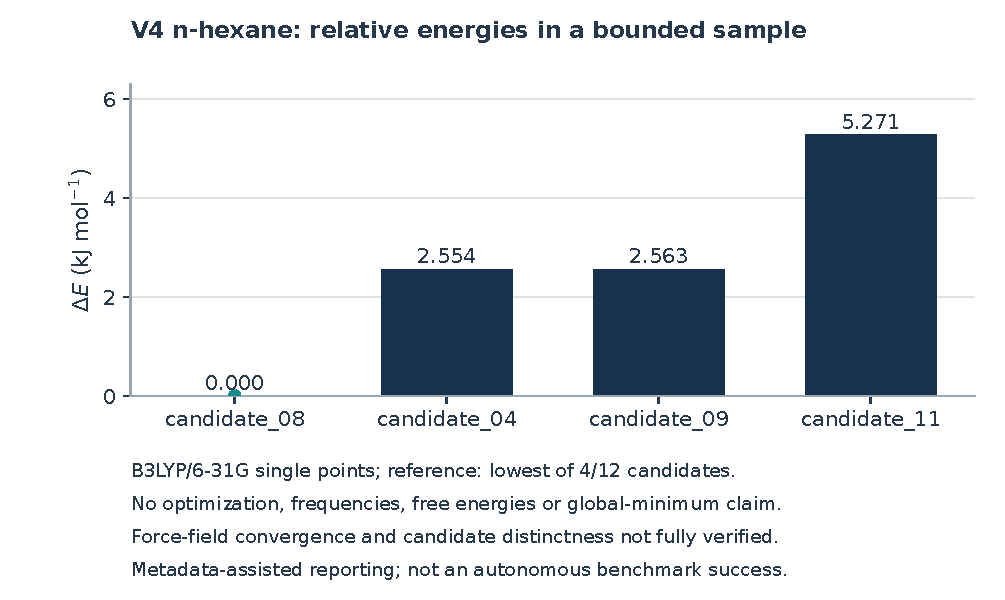
\includegraphics[width=0.94\linewidth]{bounded-conformers.pdf}
\caption{V4 正己烷有限候选的单点相对电子能。四个已评估候选相对于子集最低值为 0、2.554112、2.563181、5.270516 kJ mol$^{-1}$。另八个候选未进行 ORCA 计算，所得顺序不代表全局构象、自由能或极小值排序。}
\label{fig:conformers}
\end{figure}

任务代码与科学计算来自模型驱动过程，最终证据组织与交付包含人工元数据协助及分次续作。相关运行累计 38 次模型请求、854,725 tokens 和 4 次 ORCA 计算，不能计入完全自主冻结评测的成功样本。候选间完全互异与力场收敛也未充分验证。本例支持预算内有限候选比较的可行性，其证据边界不同于全局构象搜索。四次 ORCA 单点均作为计算成功记录。

% !TeX root = ../main.tex
\subsection{已成功计算的任务与数值结果}
\label{sec:successful-results}
为完整呈现实际计算产出，本节进一步汇总后续修复实验及历史批次中的成功计算。本文将原始输出含 ORCA 正常结束记录的调用标注为\textbf{计算成功}，并另行说明收敛、几何及性质解释的证据范围。T1--T5 与 H1 六类任务已有数值结果，H2 尚无极化率结果。这里的六类覆盖来自不同配置与多次开发尝试，不能解释为同一版本七题一次运行的成功率；它也不改变各历史批次的原始工作流完成记录。

\begin{table}[htbp]
\centering\small
\caption{V4 已获数值结果的任务覆盖。成功按实际 ORCA 调用判断，附加说明限定结论范围。}
\label{tab:successful-coverage}
\begin{tabularx}{\linewidth}{p{0.9cm}p{2.2cm}p{2.2cm}Y}
\toprule
任务 & 计算状态 & 主要批次 & 已获得结果\\
\midrule
T1 & 计算成功 & a010 & 乙醇优化能量、收敛结构与 21 个正频率\\
T2 & 计算成功 & a005、a007 & 两批共 10 个候选的单点能量及批内排序\\
T3 & 计算成功（部分点） & 第三冻结批次 & 六个约束优化计算点；角度对应待核查\\
T4 & 计算成功 & 第一冻结批次 & 丙酮五个单重态激发能及振子强度\\
T5 & 计算成功 & a026、a027 & 两种基组下各一对气相与 CPCM 水能量\\
H1 & 计算成功 & a011 & 三核总屏蔽张量及各向同性屏蔽\\
H2 & 尚无计算结果 & 已有记录 & 未获得两个取向的静态极化率\\
\bottomrule
\end{tabularx}
\end{table}

\subsubsection{T1：乙醇优化与振动频率}
批次 a010 使用气相 r$^{2}$SCAN-3c 及其内置 def2-mTZVPP 基组，电荷为 0、多重度为 1。ORCA 计算成功，优化的五项数值收敛阈值均满足，最终电子能为 $-155.002345492244\,\Eh$。27 个模式中包含投影后的 6 个平动和转动零模式、21 个正振动模式及 0 个虚频。全部正频率见表 \ref{tab:t1-frequencies}。这些结果支持该理论水平下的局部极小值，不证明全局最低构象。

\begin{table}[htbp]
\centering\small
\caption{a010 乙醇的 21 个正振动频率，单位 cm$^{-1}$，按 ORCA 打印精度列示。}
\label{tab:t1-frequencies}
\begin{tabular}{rrrrrrr}
\toprule
270.90 & 298.95 & 425.86 & 811.51 & 882.13 & 1052.13 & 1066.45\\
1134.41 & 1282.25 & 1371.13 & 1396.18 & 1418.25 & 1483.33 & 1487.57\\
1509.53 & 2969.59 & 3004.65 & 3061.83 & 3088.36 & 3105.66 & 3819.31\\
\bottomrule
\end{tabular}
\end{table}

\subsubsection{T2：正己烷有限候选的单点能量}
a007 和 a005 分别完成 6 次与 4 次气相 r$^{2}$SCAN-3c 单点计算，均为中性单重态。表 \ref{tab:t2-energies} 给出真实电子能及相对能量；每批以各自已计算子集的最低能量为参考，换算采用 $1\,\Eh=2625.4996394799$ kJ mol$^{-1}$。候选编号只在批次内部有效，相同编号不能视为同一结构。结果支持有限几何集合的单点排序，不能称为全部候选均经 DFT 优化，也不构成全局构象或自由能排序。

\begin{table}[htbp]
\centering\small
\caption{正己烷两批成功单点计算。相对能量在各批内部定义。}
\label{tab:t2-energies}
\begin{tabular}{llrr}
\toprule
批次 & 候选 & 电子能 / $\Eh$ & 相对能量 / kJ mol$^{-1}$\\
\midrule
a005 & cand\_47 & $-236.992098209035$ & 0.000000\\
a005 & cand\_26 & $-236.991452622119$ & 1.694988\\
a005 & cand\_05 & $-236.991445556634$ & 1.713539\\
a005 & cand\_02 & $-236.991444090374$ & 1.717388\\
\addlinespace
a007 & cand\_05 & $-236.992066202851$ & 0.000000\\
a007 & cand\_04 & $-236.991445556657$ & 1.629506\\
a007 & cand\_01 & $-236.991444090308$ & 1.633356\\
a007 & cand\_00 & $-236.991421448668$ & 1.692802\\
a007 & cand\_06 & $-236.991245997872$ & 2.153448\\
a007 & cand\_03 & $-236.987263819406$ & 12.608656\\
\addlinespace
\bottomrule
\end{tabular}
\end{table}

\subsubsection{T3：正丁烷约束优化的六个计算点}
第三冻结批次使用气相 r$^{2}$SCAN-3c、中性单重态，完成六次约束优化；各次均有 ORCA 正常结束和优化收敛记录，因而标为计算成功。表 \ref{tab:t3-energies} 的第一列是输入目标角度标签。生成脚本报告的实际角度与标签存在矛盾，尚未通过独立几何核查确认，不能将标签直接当作已验证二面角，也不能据此确认势垒。$+120^\circ$ 标签下的高能量尤其不能直接解释为可信物理势垒；$+180^\circ$ 点未启动。

\begin{table}[htbp]
\centering\small
\caption{成功完成的六个正丁烷计算点。角度为输入标签；相对电子能以这六个点中的最低值为零。}
\label{tab:t3-energies}
\begin{tabular}{rrr}
\toprule
输入标签 / $^\circ$ & 电子能 / $\Eh$ & 相对能量 / kJ mol$^{-1}$\\
\midrule
$-180$ & $-158.392470368263$ & 0.000000\\
$-120$ & $-158.387146187943$ & 13.978634\\
$-60$ & $-158.391526560891$ & 2.477966\\
$+0$ & $-158.383528626170$ & 23.476541\\
$+60$ & $-158.391526702130$ & 2.477595\\
$+120$ & $-158.358972460497$ & 87.948745\\
\bottomrule
\end{tabular}
\end{table}

较早批次还成功完成了一个 B3LYP/def2-TZVP 计算点。输入目标为 $-180^\circ$，收敛电子能为 $-158.397118300397\,\Eh$。独立读取终态几何得到 $179.999995786^\circ$，按角度周期性与目标一致。该点采用不同理论水平，不并入表 \ref{tab:t3-energies} 的相对能量。

\subsubsection{T4：丙酮五个单重态垂直激发}
第一冻结批次使用气相 PBE0/def2-SVP、中性单重态和固定准备几何，通过完整线性响应 TDDFT（TDA 关闭）成功计算五个单重激发态。SCF 和响应求解均有收敛记录，结果见表 \ref{tab:t4-excitations}。振子强度采用长度规范。后续产品解析未能提取这些行，不影响原始 ORCA 计算的成功判定；本表来自原始输出的只读核查。计划中的 CAM-B3LYP/def2-TZVP 没有实际执行，不能用作本表的方法标签。

\begin{table}[htbp]
\centering\small
\caption{丙酮前五个单重态垂直激发的实际 ORCA 输出。}
\label{tab:t4-excitations}
\begin{tabular}{rrrr}
\toprule
态 & 激发能 / eV & 波长 / nm & 振子强度 $f$\\
\midrule
$S_{1}$ & 4.197061 & 295.4 & 0.000007493\\
$S_{2}$ & 7.464499 & 166.1 & 0.023781213\\
$S_{3}$ & 8.406988 & 147.5 & 0.001899769\\
$S_{4}$ & 8.572306 & 144.6 & 0.060276158\\
$S_{5}$ & 8.640904 & 143.5 & 0.004121254\\
\bottomrule
\end{tabular}
\end{table}

\subsubsection{T5：固定几何下的气相与水环境电子能量}
a026 和 a027 均使用 B3LYP、中性单重态；每批气相与 CPCM 水计算使用完全相同的初始几何和原子顺序，分别完成两次 ORCA 计算。该几何不是 T1 优化后的结构。表 \ref{tab:t5-environments} 按实际基组分开报告，以 $\Delta E=E_{\mathrm{water}}-E_{\mathrm{gas}}$ 定义差值。两批结果均为负，表示指定模型与几何下水环境电子能较低；这是电子能量差，不是水合自由能。

\begin{table}[htbp]
\centering\small
\caption{两批气相与 CPCM 水环境的成功单点计算。能量单位为 $\Eh$，最后一列为 kJ mol$^{-1}$。}
\label{tab:t5-environments}
\begin{tabular}{lrrrr}
\toprule
批次 / 基组 & $E_{\mathrm{gas}}$ & $E_{\mathrm{water}}$ & $\Delta E$ & $\Delta E$\\
\midrule
a026 / def2-TZVP & $-155.002778990957$ & $-155.009740144896$ & $-0.006961153939$ & $-18.276507$\\
a027 / def2-SVP & $-154.817054999208$ & $-154.823380641772$ & $-0.006325642564$ & $-16.607972$\\
\bottomrule
\end{tabular}
\end{table}

\subsubsection{H1：HCN 的 GIAO 核磁屏蔽张量}
a011 在固定初始几何上采用气相 PBE0/def2-TZVP、中性单重态及 GIAO，ORCA 计算成功，总电子能为 $-93.345070922944\,\Eh$。按原子顺序 C$_0$、N$_1$、H$_2$，各向同性屏蔽分别为 79.051、$-34.068$ 和 29.850 ppm。完整笛卡尔总屏蔽张量如下，行列顺序为 X、Y、Z，单位 ppm，保留原始三位小数：
\begin{equation}
\bm{\sigma}_{\mathrm{C}_0}=\begin{pmatrix}
279.306 & -0.724 & -0.000 \\
-1.638 & -21.077 & 0.000 \\
-0.000 & 0.000 & -21.076
\end{pmatrix}.
\end{equation}
\begin{equation}
\bm{\sigma}_{\mathrm{N}_1}=\begin{pmatrix}
340.398 & -1.842 & -0.000 \\
-0.044 & -221.291 & 0.000 \\
0.000 & 0.000 & -221.309
\end{pmatrix}.
\end{equation}
\begin{equation}
\bm{\sigma}_{\mathrm{H}_2}=\begin{pmatrix}
39.712 & 0.055 & -0.000 \\
-0.114 & 24.919 & -0.000 \\
-0.000 & -0.000 & 24.920
\end{pmatrix}.
\end{equation}
各向同性屏蔽定义为 $\sigma_{\mathrm{iso}}=\mathrm{Tr}(\bm\sigma)/3$，与打印摘要在舍入精度内一致。上述量为绝对屏蔽，未引入参考物质，不能直接称为实验化学位移。张量非对角元按原始输出保留，不作未经说明的对称化。

\subsubsection{H2：静态极化率的结果状态}
甲醛两个取向的静态极化率张量、各向同性值及旋转一致性比较尚未得到实际 ORCA 数值，因此本项标为\textbf{尚无计算结果}。准备的几何和旋转方案不计为成功科学计算。


\subsection{冻结批次的计算成功与成本}
在表 \ref{tab:v4-settings} 的配置下，七任务评测共发生 53 次模型调用、1,048,678 tokens 和 8 次实际 ORCA 启动，其中 7 次计算成功，已启动调用的成功比例为 $7/8=87.5\%$。T3 的六次和 H1 的一次成功计算均保留为正面成果；T4 的一次为输入失败，另外四题未启动。表 \ref{tab:v4-tasks} 与图 \ref{fig:v4-tasks} 给出该固定批次的计算状态与成本。该批次的全部必需目标交付为 0/7，这一附加指标不用于否定已经成功的 ORCA 计算。

\begin{table}[htbp]
\centering\small
\caption{原冻结批次的 ORCA 计算结果。调用成功与任务后处理分开记录。}
\label{tab:v4-tasks}
\begin{tabularx}{\linewidth}{p{1.0cm}rrrY}
\toprule
任务 & 模型调用 & tokens & 启动/成功 & 计算状态与后续处理\\
\midrule
T1 & 3 & 39,588 & 0/0 & 未计算；规范化阶段停止\\
T2 & 3 & 36,542 & 0/0 & 未计算；响应与目标表达未被接受\\
T3 & 14 & 338,495 & 6/6 & 计算成功；角度核查及完整扫描交付待完善\\
T4 & 16 & 343,256 & 1/0 & 计算失败；ORCA 输入关键词错误\\
T5 & 3 & 34,966 & 0/0 & 未计算；条件传递阶段停止\\
H1 & 11 & 207,725 & 1/1 & 计算成功；三核张量已生成，后处理未完成\\
H2 & 3 & 48,106 & 0/0 & 未计算；语义纠正额度耗尽\\
\midrule
合计 & 53 & 1,048,678 & 8/7 & 已启动调用的计算成功比例 87.5\%\\
\bottomrule
\end{tabularx}
\end{table}

\begin{figure}[htbp]
\centering
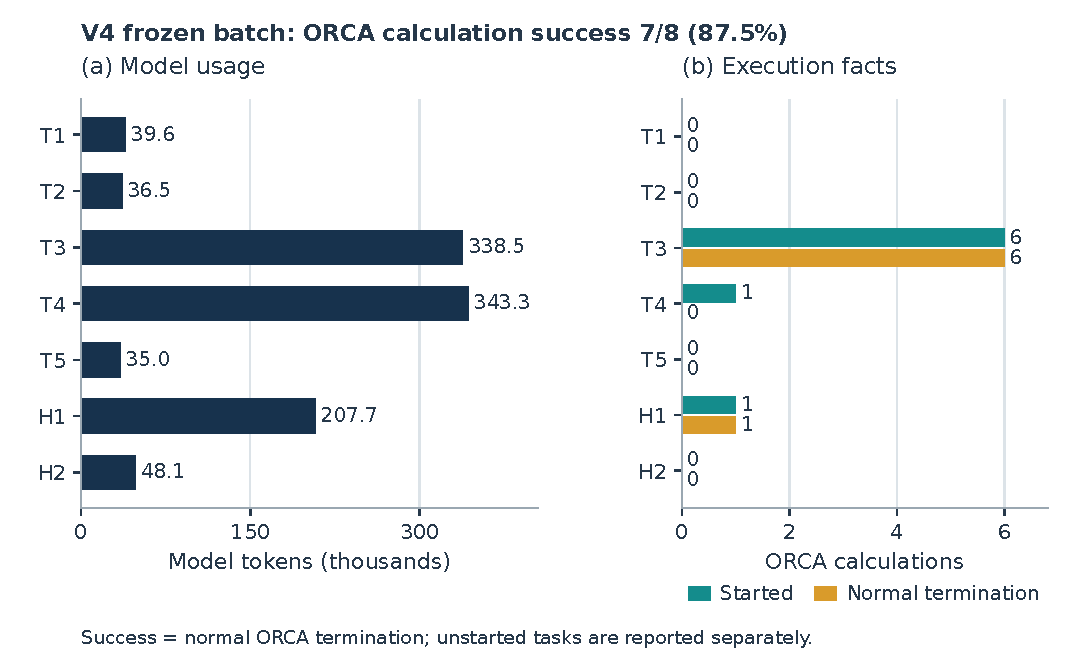
\includegraphics[width=\linewidth]{latest-tasks.pdf}
\caption{V4 七任务评测的模型 token 用量与 ORCA 执行事实。7 次计算成功来自 T3 六次和 H1 一次，另有 1 次 ORCA 输入失败。}
\label{fig:v4-tasks}
\end{figure}

T3 最能说明运行成功与目标完成的分离。模型修复一次 Python 格式化错误后，六次内部 ORCA 计算正常结束并保存产物。然而，程序自设的时间窗口跳过 $+180^\circ$ 端点，曲线与后续采样加密决定没有完成；实际角度与目标角度也未被独立重算。随后反馈上下文超限，且修复步骤未完整继承原目标路线。因此，即使内部计算正常结束，也缺少支持完整扫描结论的证据。

H1 的 NMR 计算产生了 C、N、H 三核总屏蔽张量及各向同性摘要，但结果返回后的上下文构建失败，使后续提取和核对无法完成。T4 则因 ORCA 输入关键词错误停止，外层程序异常掩盖内部错误信息，模型未能及时定位有效修复入口。其中 H1 的 ORCA 计算成功，后续处理失败应单独归因；T4 则属于 ORCA 输入失败。证据发现和结果消费仍是闭环性能的重要组成部分。

\subsection{成本与跨配置观察}
七任务主评测的执行驱动累计经过时间为 2706.749 s，记录的科学计算经过时间和 CPU 时间分别为 1178.063 s 与 3581.138406 s；因采样覆盖有限，后二者作为观测下界。按实验价表计算的模型费用上界为 0.5735982 USD，不代表实际结算账单。模型成本还包含重复读取和反馈组织，不能将 token 用量直接解释为有效科学推理量。

\begin{figure}[htbp]
\centering
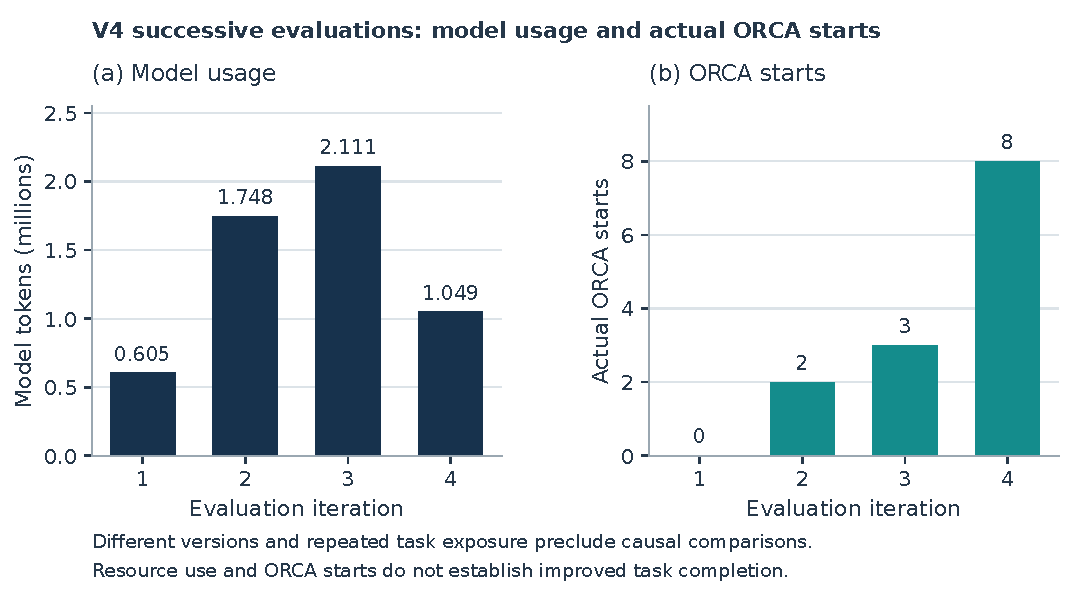
\includegraphics[width=0.96\linewidth]{evaluation-history.pdf}
\caption{V4 四个实验配置的模型 token 用量与 ORCA 启动数。每配置均对相同七题各进行一次评测，配置和任务暴露程度变化，启动次数不直接代表成功次数，故该图仅作描述性统计。}
\label{fig:v4-configurations}
\end{figure}

四个不同配置累计发生 294 次模型调用、5,512,391 tokens 和 13 次 ORCA 启动，完整完成为 0/28 次任务尝试。它们不是同一版本的 28 次独立试验，也不能与 V3 的情境评分合并。历史工作流完成记录作为补充事实保存；本文的计算成果以正常结束调用及其实际数值为依据。后续开发批次已有表 \ref{tab:successful-coverage} 所列六类数值产出，不将其与上述四个冻结配置合并计算成功率。
